\documentclass{standalone}

\usepackage{amssymb}
\usepackage{amsthm}
\usepackage{amsmath}


\usepackage{tikz}
\usetikzlibrary{shapes,backgrounds,calc,patterns}
\usepackage{venndiagram}


\begin{document}
    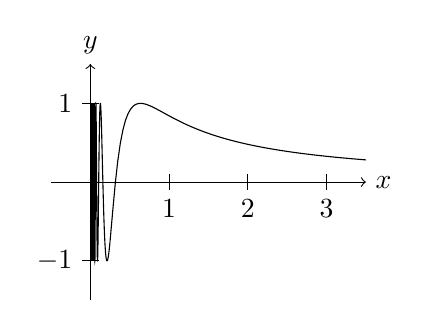
\begin{tikzpicture}
\draw[->] (-.5,0) -- (3.5,0) node[right] {\(x\)};
\draw[->] (0,-1.5) -- (0,1.5) node[above] {\(y\)};
\foreach \x in  {1,2,3}
\draw[shift={(\x,0)},color=black] (0pt,3pt) -- (0pt,-3pt);
\foreach \x in {1,2,3}
\draw[shift={(\x,0)},color=black] (0pt,0pt) -- (0pt,-3pt) node[below] {\(\x\)};
\foreach \x in {-1,1}
\draw[shift={(0,\x)},color=black] (-3pt,0pt) -- (3pt,0pt);
\foreach \x in {-1,1}
\draw[shift={(0,\x)},color=black] (0pt,0pt) -- (-3pt,0pt) node[left] {\(\x\)};
\draw[black,domain=0.01:.25,samples=1000] plot (\x, {sin((1/\x)r)});
\draw[black,domain=.25:3.5,samples=100] plot (\x, {sin((1/\x)r});
\end{tikzpicture}
\end{document}